\documentclass[dvipdfmx]{jarticle}
\usepackage[paperwidth=594mm,paperheight=841mm,
            top=18mm,bottom=18mm,left=18mm,right=18mm]{geometry}
\usepackage{graphicx}
\usepackage{booktabs}
\usepackage{color}
\usepackage{amsmath,amssymb}
\usepackage{enumitem}
\pagestyle{empty}

%% dvipdfmx に用紙サイズを伝える
\AtBeginDvi{\special{papersize=594mm,841mm}}

%% カラー定義
\definecolor{titleblue}{rgb}{0.10,0.22,0.46}
\definecolor{secblue}{rgb}{0.16,0.36,0.64}
\definecolor{accentred}{rgb}{0.78,0.10,0.10}
\definecolor{staryellow}{rgb}{1.0,0.85,0.0}
\definecolor{darkgreen}{rgb}{0.0,0.50,0.0}
\definecolor{lightyellow}{rgb}{1.0,0.97,0.85}

%% セクションヘッダ（大型化）
\newcommand{\sechead}[1]{%
  \par\noindent
  \colorbox{secblue}{\textcolor{white}{\Large\textbf{\,#1\,}}}\\[3mm]%
}

%% 図キャプション
\newcommand{\figcap}[1]{{\normalsize\textbf{#1}}}

\begin{document}
\fontsize{22}{30}\selectfont

%% ════════════════════════════════════════════
%% ヘッダー（フル幅）
%% ════════════════════════════════════════════
\noindent
\colorbox{titleblue}{\parbox{\dimexpr\linewidth-2\fboxsep\relax}{%
  \centering\vspace{4mm}%
  \textcolor{white}{\fontsize{40}{50}\selectfont\textbf{%
    教師なし物体セグメンテーションによる\\[2mm]
    金属光沢面の認識可能性の検討}}\\[3mm]
  \textcolor{white}{\fontsize{24}{30}\selectfont%
    --- 凍結ViT 3種バックボーン比較と Goldilocks 特性の同定 ---}\\[3mm]
  \textcolor{white}{\fontsize{22}{28}\selectfont%
    坂口 健（電気通信大学）\qquad 中世 大雄（東京大学）}\vspace{4mm}%
}}

\vspace{5mm}

%% ════════════════════════════════════════════
%% 本文（2段組）
%% ════════════════════════════════════════════
\noindent
\begin{minipage}[t]{0.487\linewidth}

%% ── 左カラム ─────────────────────────────────

\sechead{1.\ 背景と目的}

\textbf{研究の動機}
\begin{itemize}[noitemsep,topsep=1mm]
\item 工業検査・ロボット把持で\textbf{金属光沢面の認識}は難課題
\item 鏡面反射：照明変化で外観が大きく変化 $\Rightarrow$ 物体分離が困難
\item 教師なし物体中心学習（OCL）はラベル不要で物体を自動分離
\item \textbf{DINOSAUR}：凍結ViT特徴の再構成でSlot Attentionを訓練
\end{itemize}

\vspace{2mm}
\colorbox{lightyellow}{\parbox{\dimexpr\linewidth-2\fboxsep\relax}{%
  \textbf{課題設定}：金属光沢面を含む複雑なシーンで物体を正しく分離するには，\\
  \hspace*{2em}どのViTバックボーンが最適か？\quad スロット数$K$はどう影響するか？}}

\vspace{3mm}

\sechead{2.\ 手法と実験設定}

\begin{center}
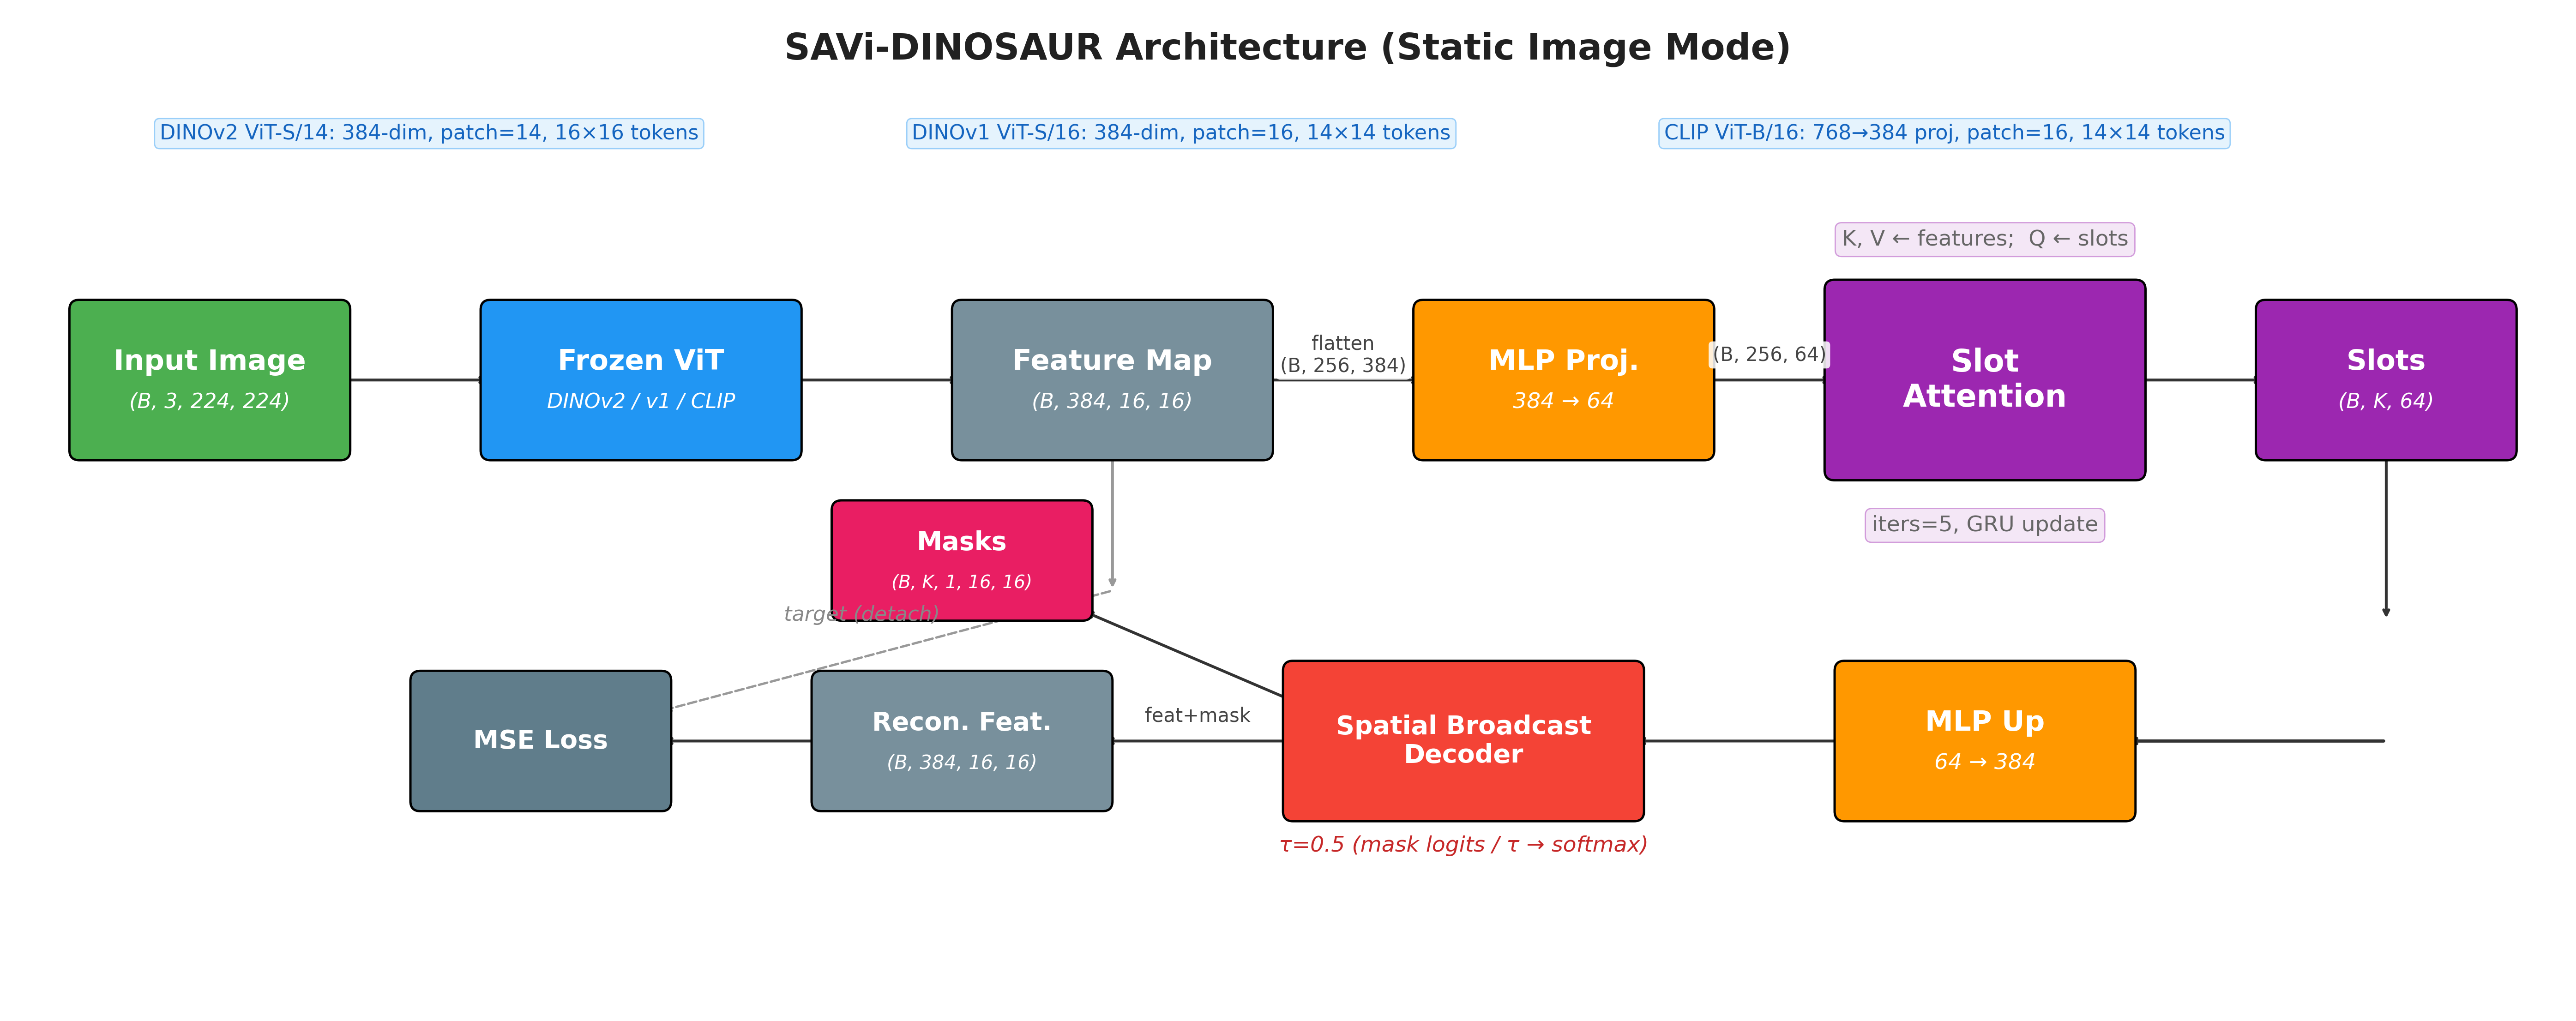
\includegraphics[width=\linewidth,keepaspectratio]{figures/architecture_diagram.png}\\[1mm]
\figcap{図1: SAVi-DINOSAURアーキテクチャ．凍結ViT $\to$ 2層MLP(384$\to$64) $\to$ Slot Attention($K$スロット) $\to$ Decoder}
\end{center}

\vspace{1mm}
\begin{itemize}[noitemsep,topsep=1mm]
\item \textbf{バックボーン}：DINOv2 ViT-S/14（自己蒸留v2），DINOv1 ViT-S/16（自己蒸留v1），CLIP ViT-B/16（画像-テキスト）
\item \textbf{データ}：MOVi-A 300シーン（金属・ゴム混在，3--10個/シーン）
\item \textbf{$K$スイープ}：$K{=}\{3,5,7,9,11,13\}$ $\times$ 3バックボーン = 18モデル
\item \textbf{評価}：FG-ARI（前景分離精度 $\uparrow$），per-object Material ARI
\end{itemize}

\vspace{3mm}

\sechead{3.\ 定量評価：$K$スイープ結果 \textcolor{staryellow}{\large$\bigstar$}}

\begin{center}
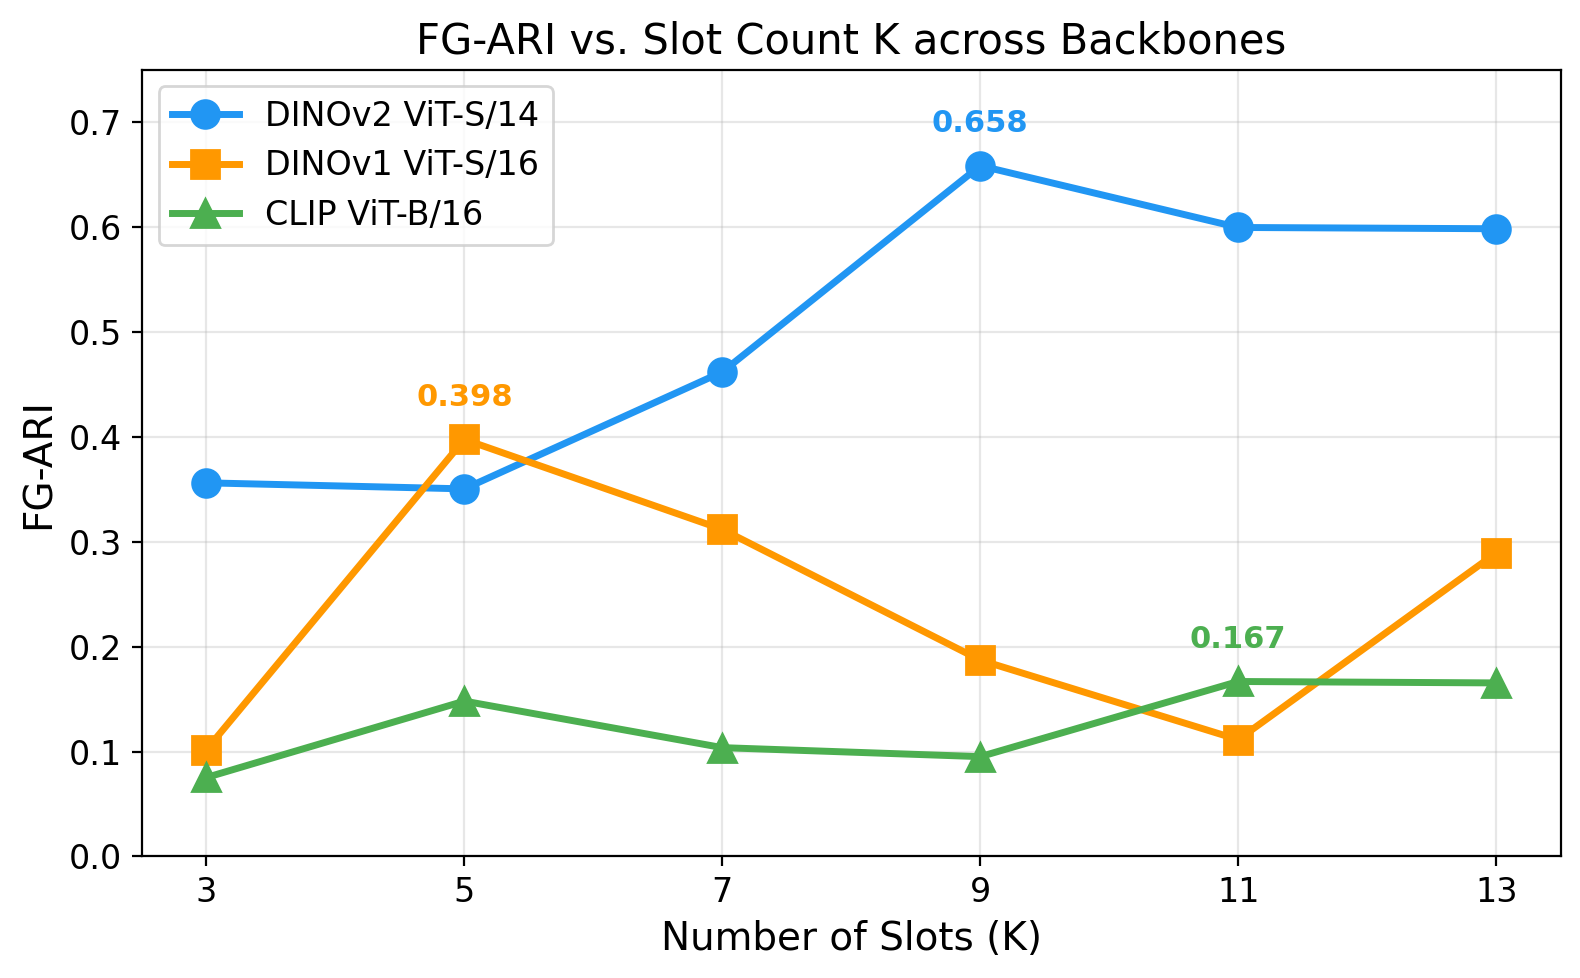
\includegraphics[width=\linewidth,keepaspectratio]{figures/k_sweep_fg_ari.png}\\[1mm]
\figcap{図2: FG-ARI vs.\ スロット数$K$．DINOv2のみ単調改善，DINOv1は急崩壊，CLIPは全$K$で低水準}
\end{center}

\begin{itemize}[noitemsep,topsep=1mm]
\item \textbf{DINOv2}：K=9でFG-ARI \textcolor{darkgreen}{\textbf{0.651}}（K=3比 $+$84\%）
\item \textbf{DINOv1}：K=5ピーク（0.403）後に急崩壊（K=11で0.107）
\item \textbf{CLIP}：全$K$で0.08--0.17，改善なし
\item 最適$K$はバックボーンごとに\textbf{質的に分岐} $\Rightarrow$ §4で原因分析
\end{itemize}

\vspace{3mm}

\sechead{4.\ Goldilocks特性：DINOv2成功の要因 \textcolor{staryellow}{\large$\bigstar$（中心的貢献）}}

\begin{center}
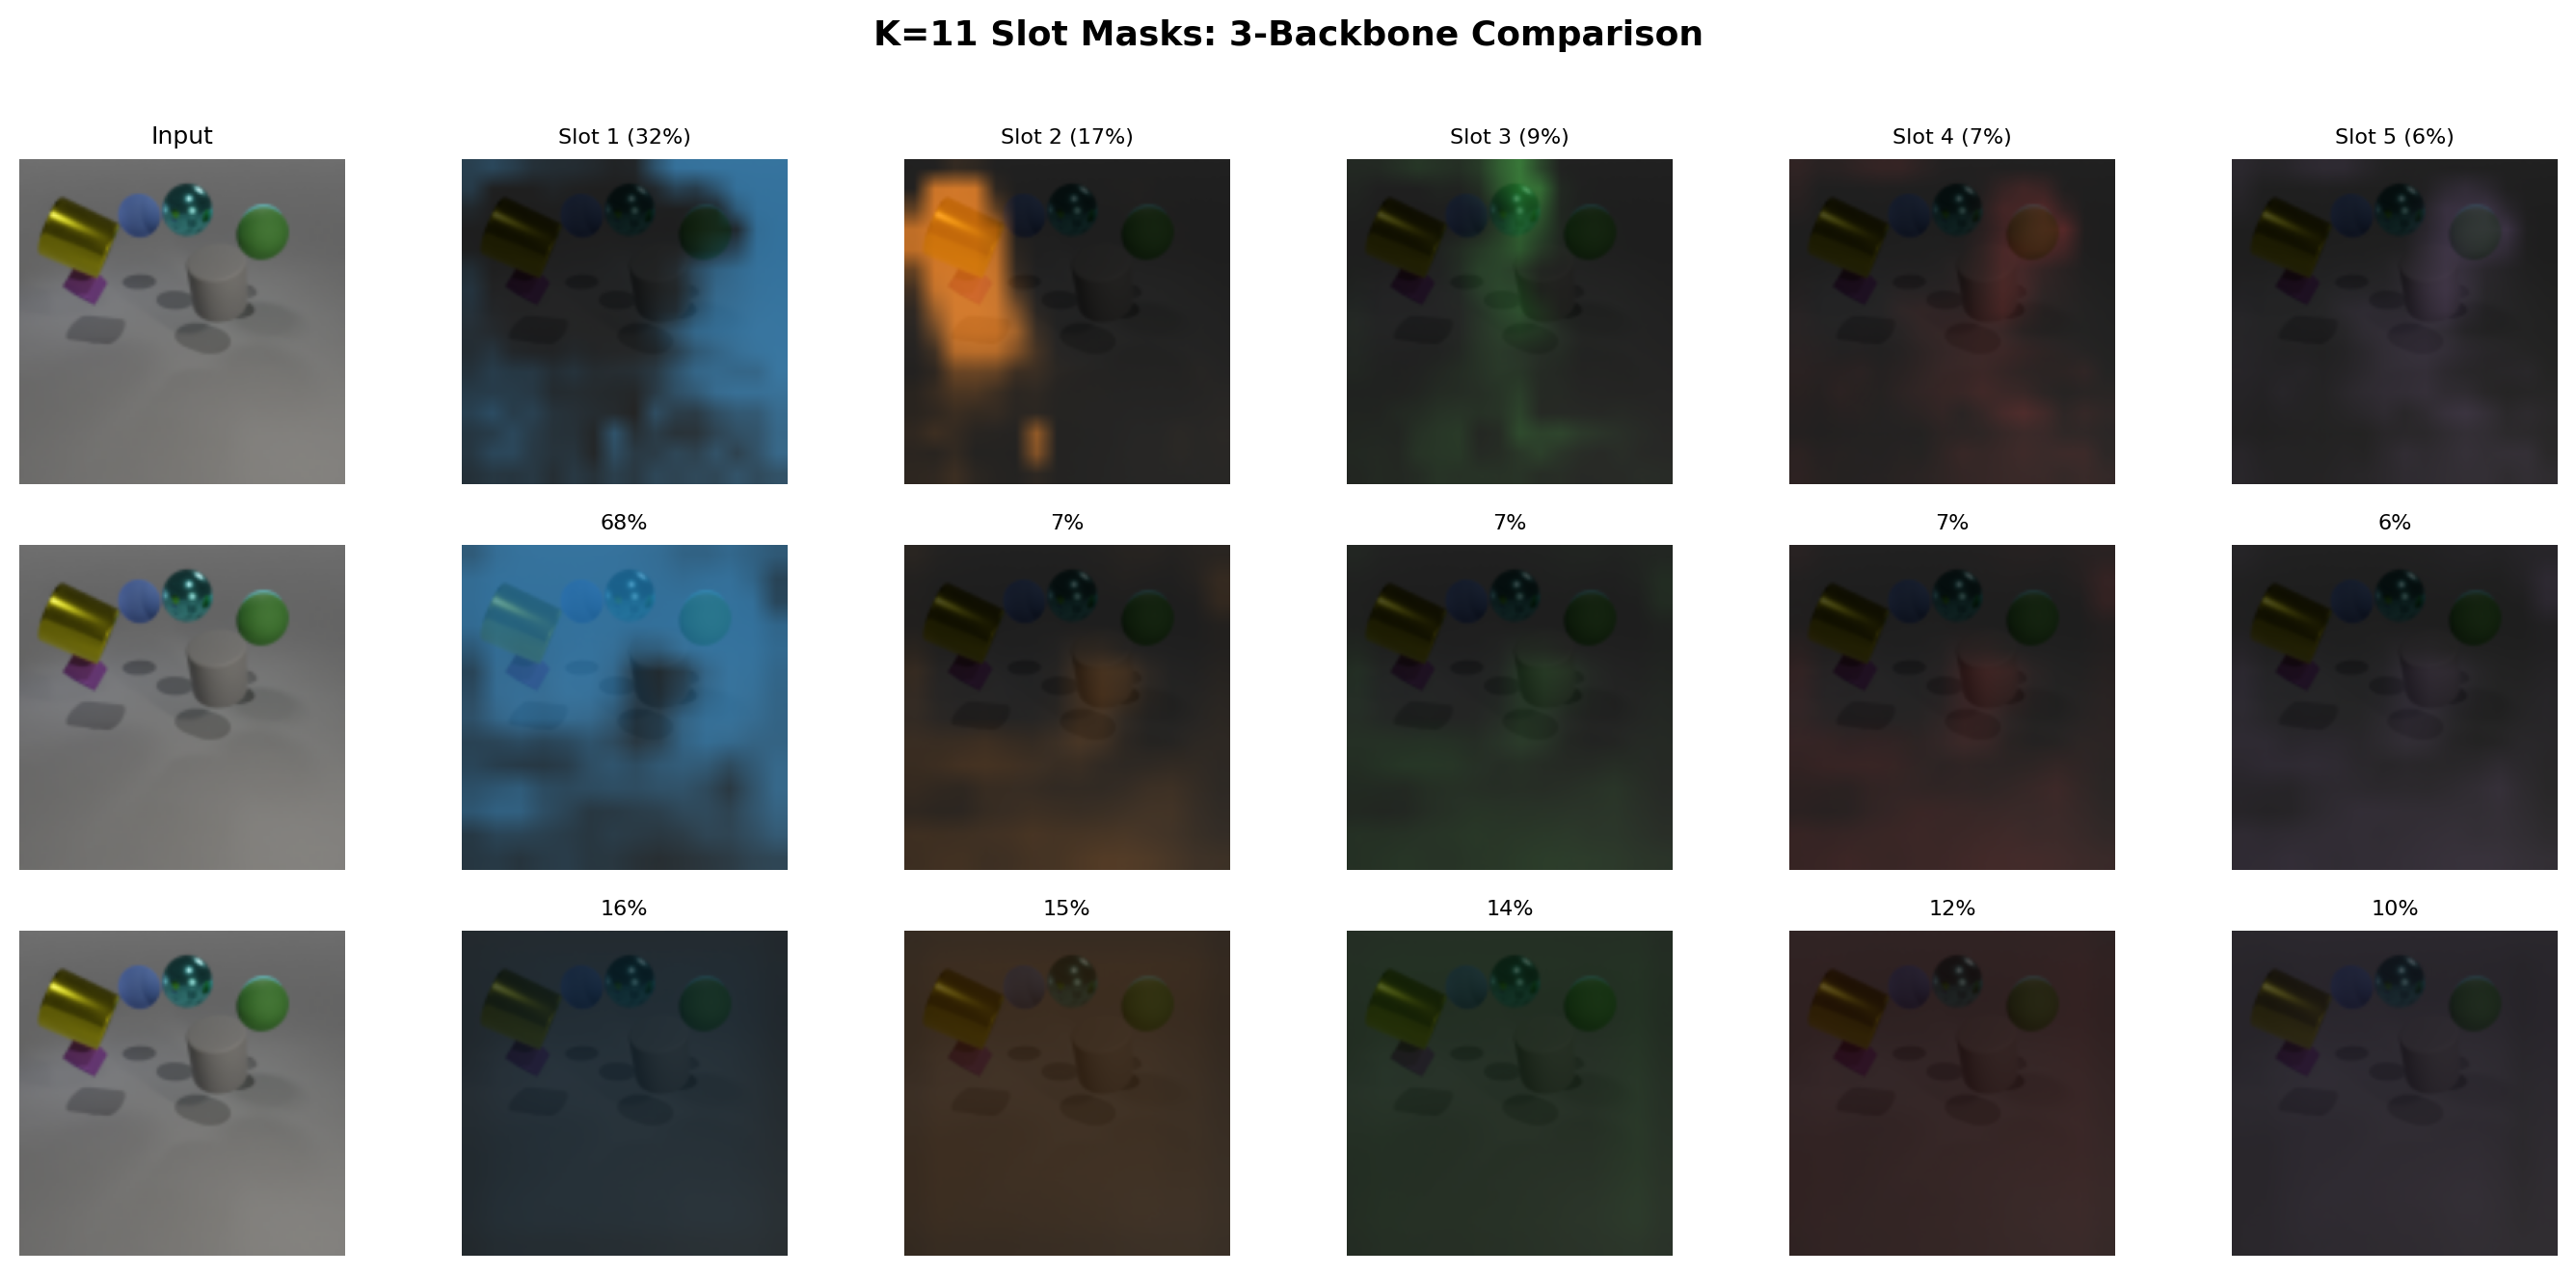
\includegraphics[width=\linewidth,keepaspectratio]{figures/poster_3backbone_k11_masks.png}\\[1mm]
\figcap{図3: K=11スロットマスク（同一シーン）．\textbf{上段 DINOv2}：物体ごとに分化 ／ \textbf{中段 DINOv1}：1スロット支配（崩壊） ／ \textbf{下段 CLIP}：全マスク均一（空間弁別なし）}
\end{center}

\vspace{1mm}
\colorbox{lightyellow}{\parbox{\dimexpr\linewidth-2\fboxsep\relax}{%
\textbf{Goldilocks特性}：DINOv2はCLIP（均一すぎ）とDINOv1（複雑すぎ）の中間\\
$\Rightarrow$ 空間多様性・情報コンパクト性・特徴スケールの3軸で\textbf{Slot Attentionに最適な中間値}}}

\vspace{2mm}
\begin{itemize}[noitemsep,topsep=1mm]
\item \textbf{CLIP失敗}：空間均一（cos=0.92）$\to$ 投影で悪化（0.99）$\to$ 自明解に収束
\item \textbf{DINOv1失敗}：PCA 45次元が64次元スロットに収まらず$\to$ 1スロット支配
\item \textbf{DINOv2成功}：PCA 20次元にコンパクト$\to$ 全11スロット分化$\to$ FG-ARI 0.651
\end{itemize}

\end{minipage}%
\hfill%
\begin{minipage}[t]{0.487\linewidth}

%% ── 右カラム ─────────────────────────────────

\sechead{5.\ 定性評価：スロット可視化}

\begin{center}
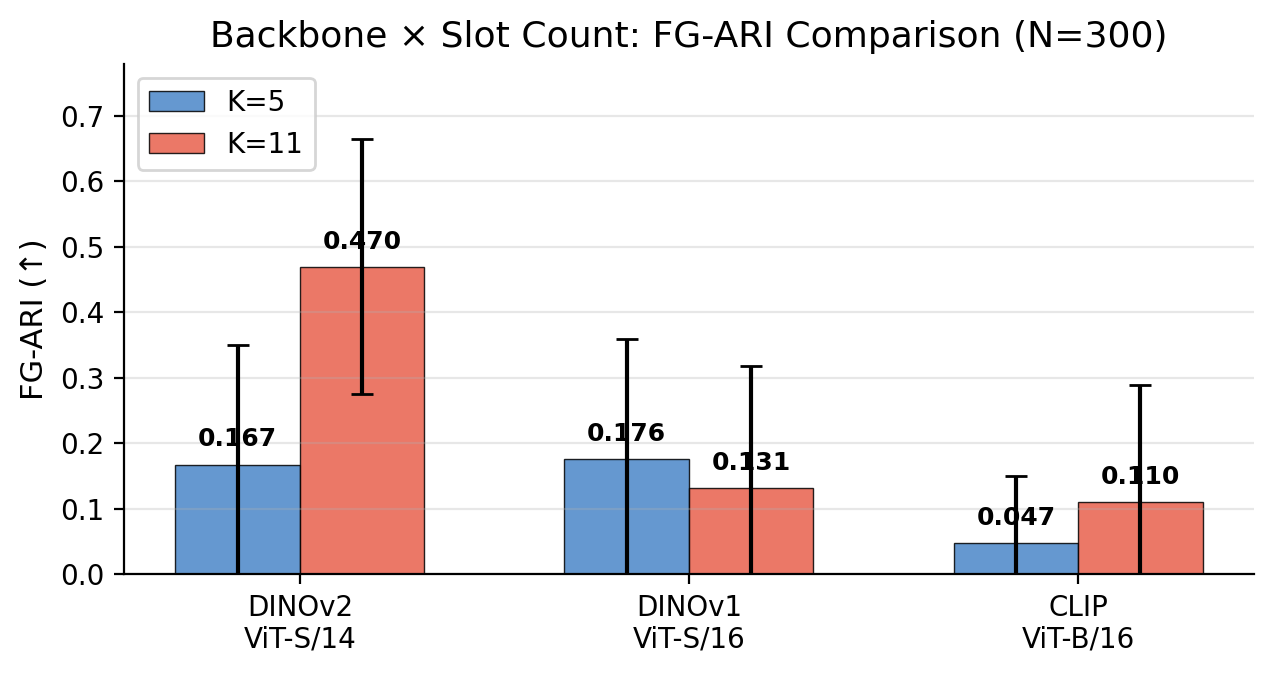
\includegraphics[width=\linewidth,keepaspectratio]{figures/poster_k5_vs_k11.png}\\[1mm]
\figcap{図4: DINOv2 K=5 vs K=11のスロットマスク比較．K=5は全スロット均一（物体未分離）$\to$ K=11は物体・背景ごとに分化達成}
\end{center}

\begin{center}
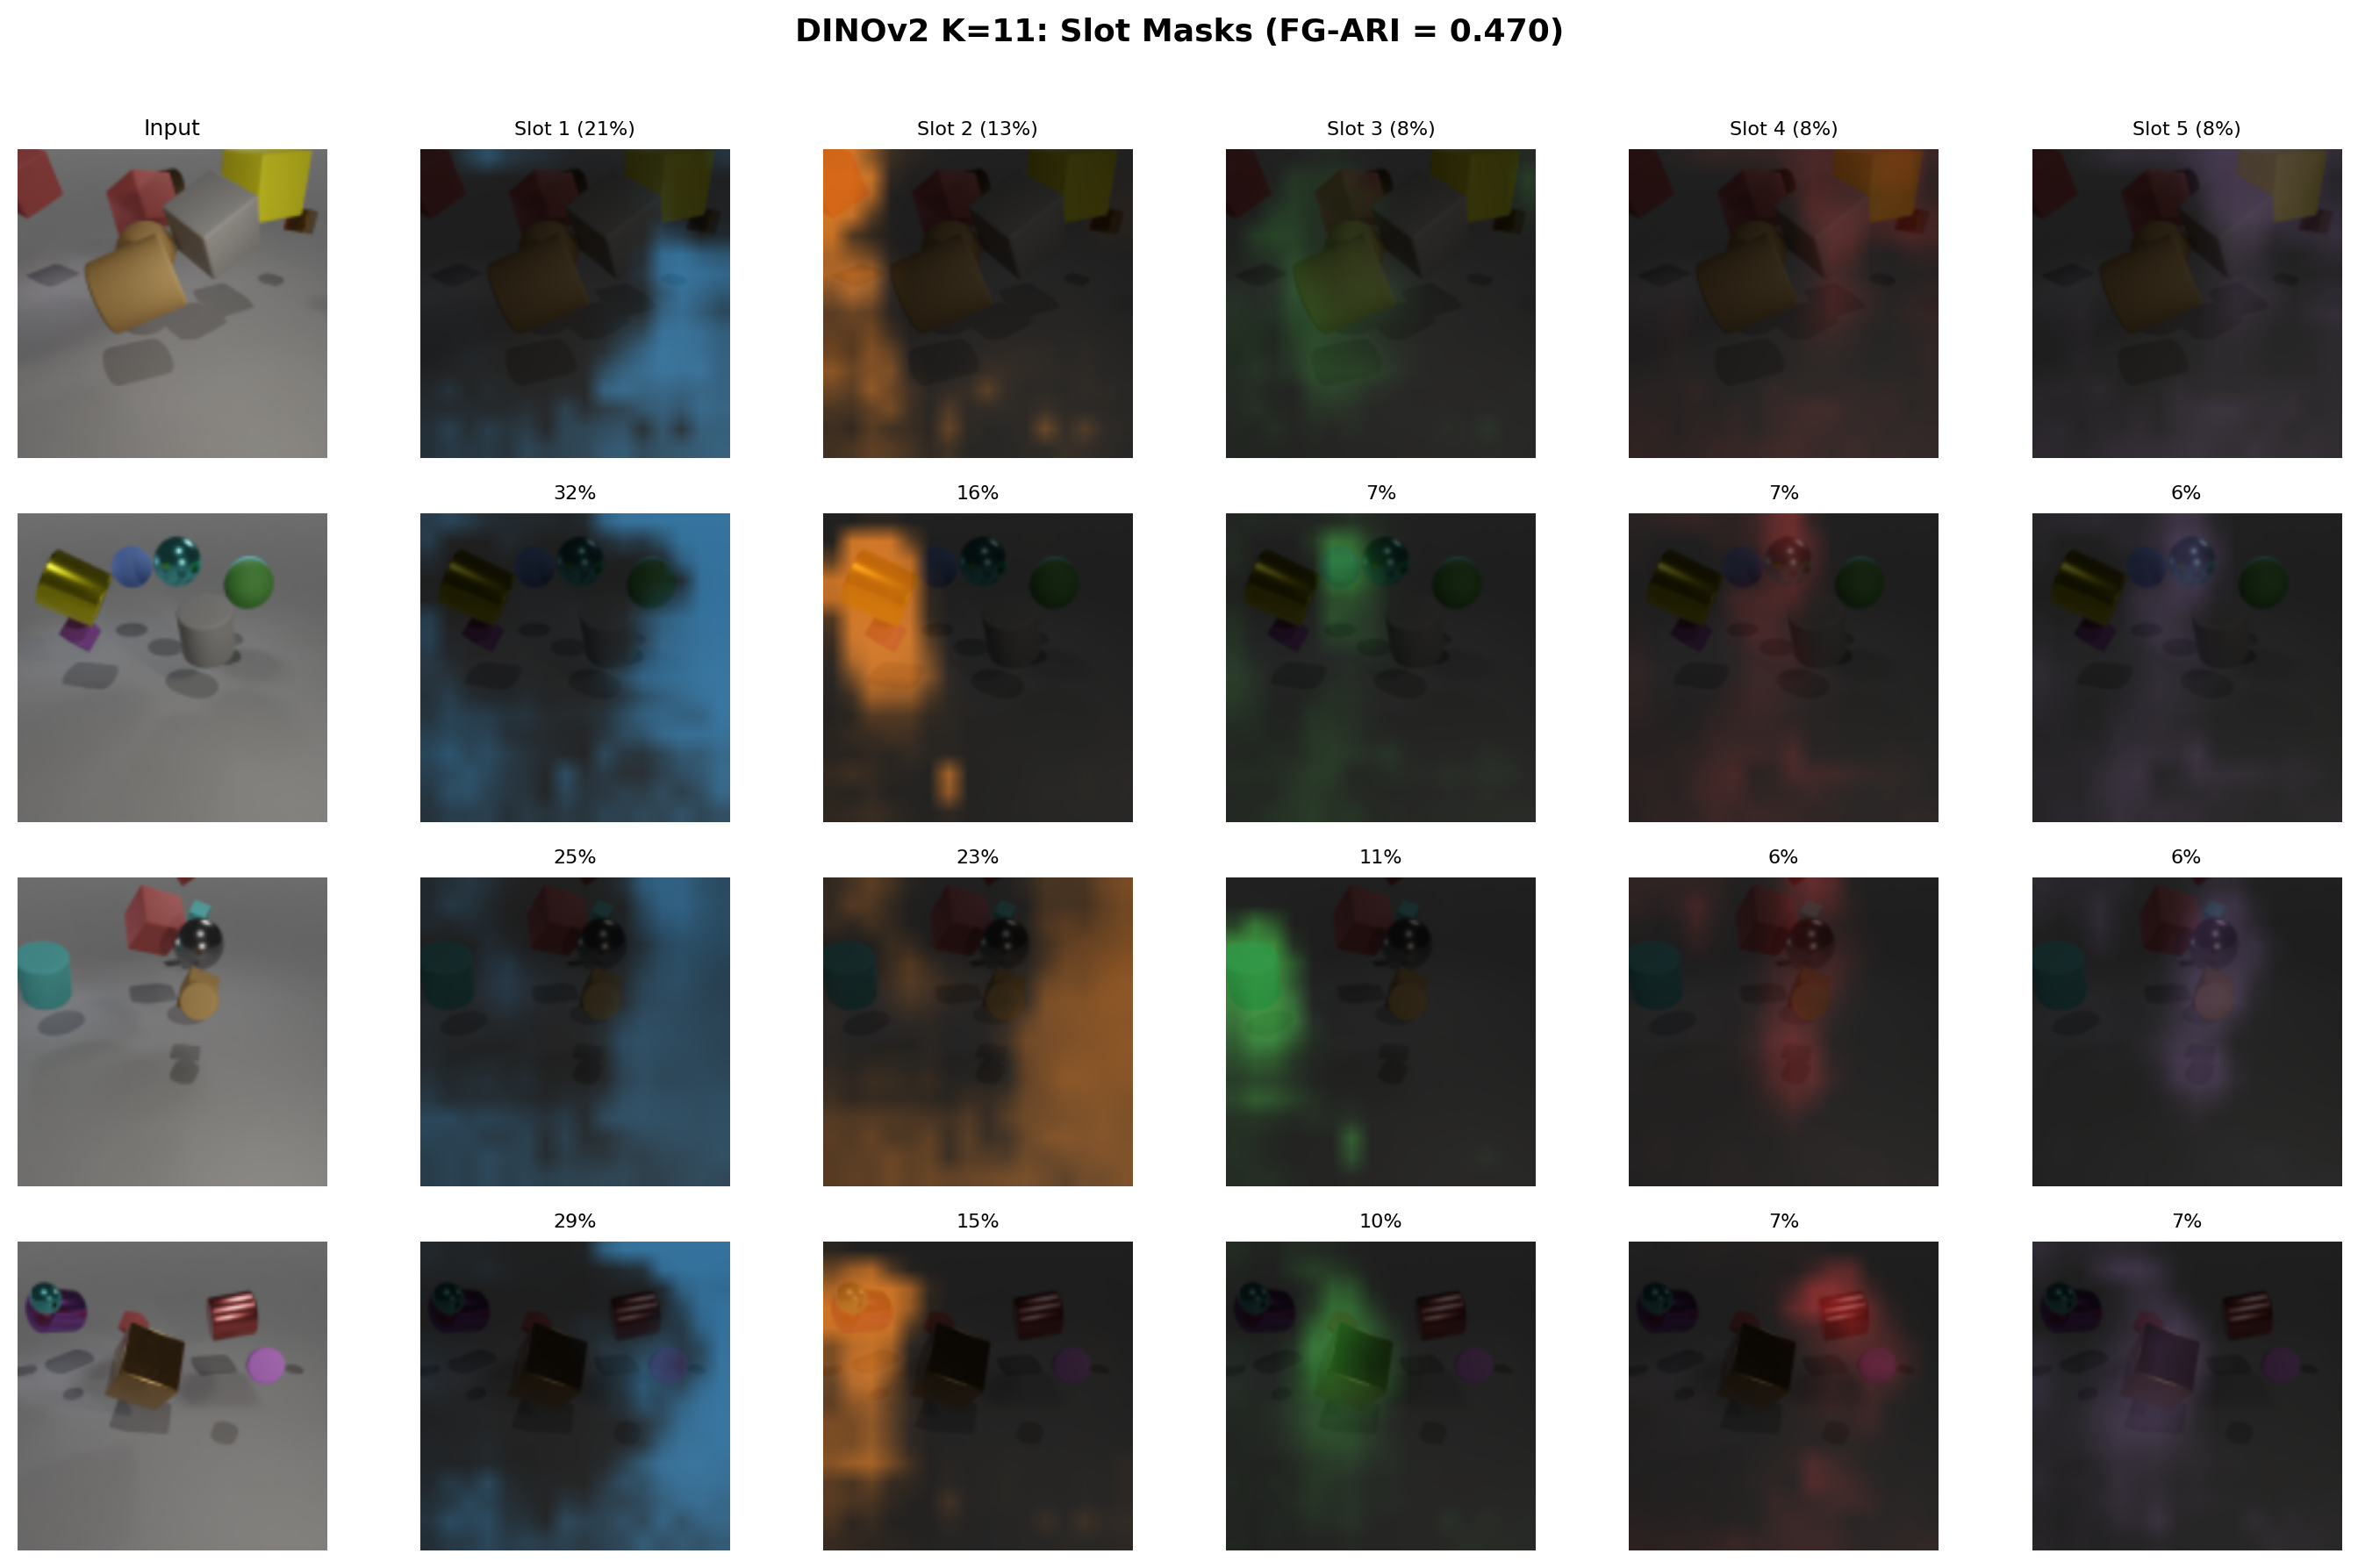
\includegraphics[width=\linewidth,keepaspectratio]{figures/poster_dinov2_k11_masks.png}\\[1mm]
\figcap{図5: DINOv2 K=11の複数シーン可視化（金属・ゴム混在）．物体数が異なるシーンでも一貫したスロット分化}
\end{center}

\vspace{1mm}
\begin{itemize}[noitemsep,topsep=1mm]
\item \textbf{16$\times$16パッチの限界}：マスク境界がにじむ $\to$ K=11でも解消しない（ViT構造的制約）
\item 金属/ゴムのMaterial ARI差：\textbf{p=0.12（有意でない）}\\
  \hspace*{1em}$\to$ スロット数確保（K=11）で部分緩和，根本解決には\textbf{動画学習が必要}
\end{itemize}

\vspace{2mm}

\sechead{6.\ $K$・$\tau$探索の概要}

\begin{center}
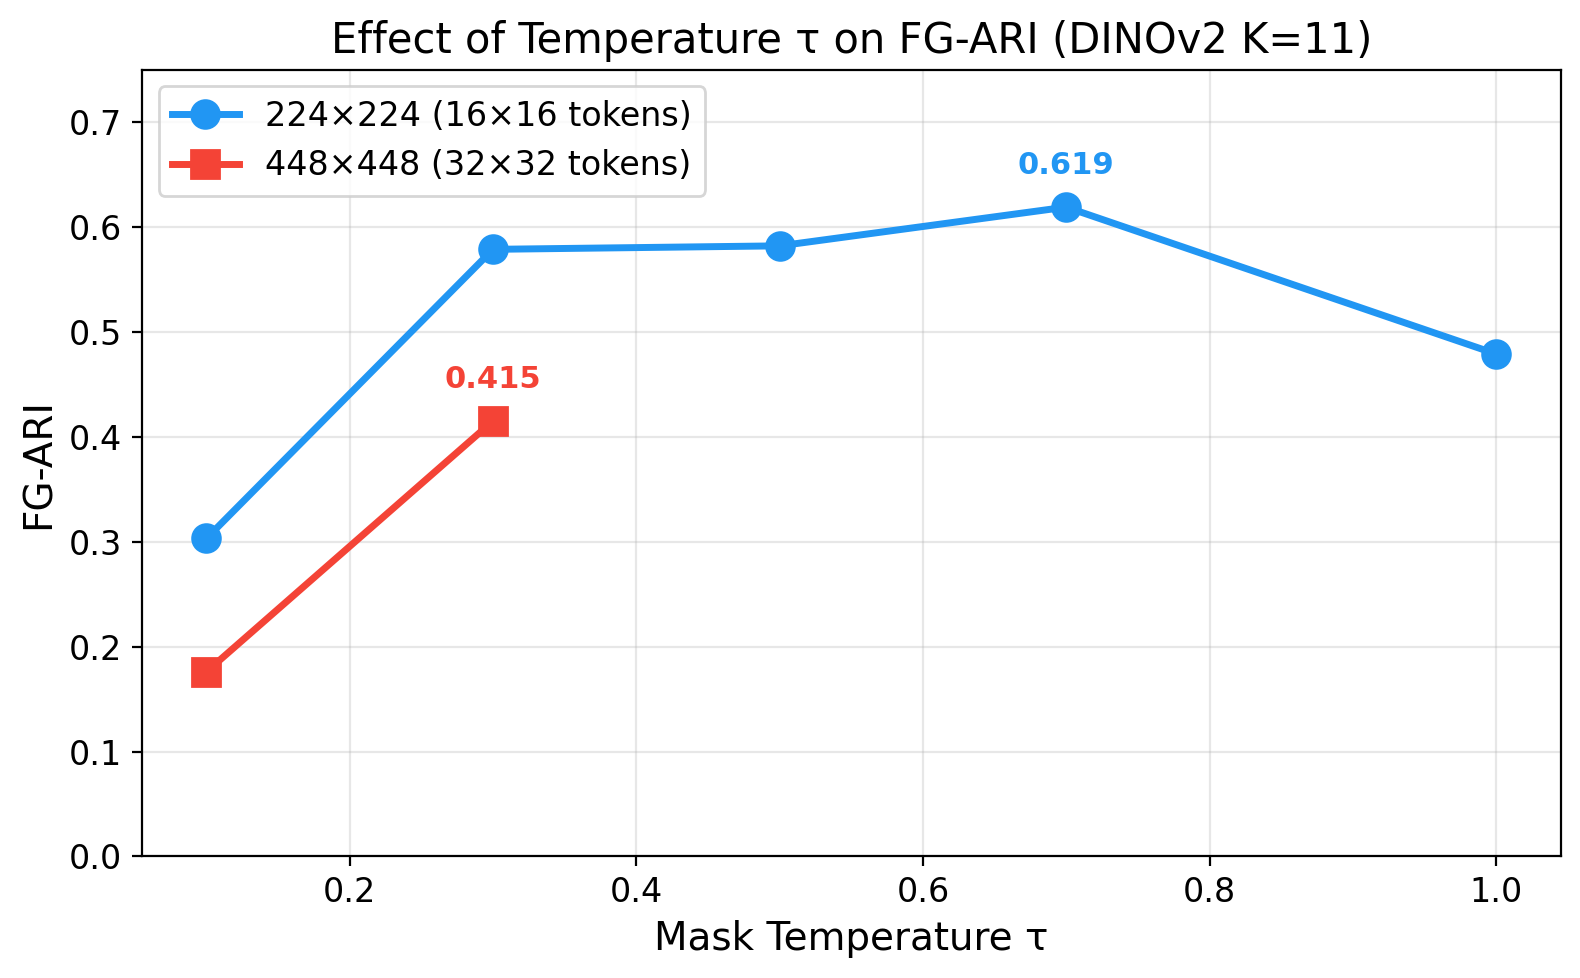
\includegraphics[width=\linewidth,keepaspectratio]{figures/tau_sweep_fg_ari.png}\\[1mm]
\figcap{図6: FG-ARI vs.\ $\tau$（DINOv2 K=11）．448px $\times$ $\tau$=0.3が全条件最良（\textbf{FG-ARI 0.696}）}
\end{center}

\begin{itemize}[noitemsep,topsep=1mm]
\item \textbf{448px $\times$ $\tau$=0.3でFG-ARI \textcolor{darkgreen}{0.696}}（全条件最良）$\to$ 高解像度では\textbf{小さい$\tau$}が必要
\item {\small 注）解像度と$\tau$が交絡 $\to$ 独立制御実験が今後の課題}
\end{itemize}

\vspace{2mm}

\sechead{7.\ マスク不確実性（エントロピー）分析}

\begin{center}
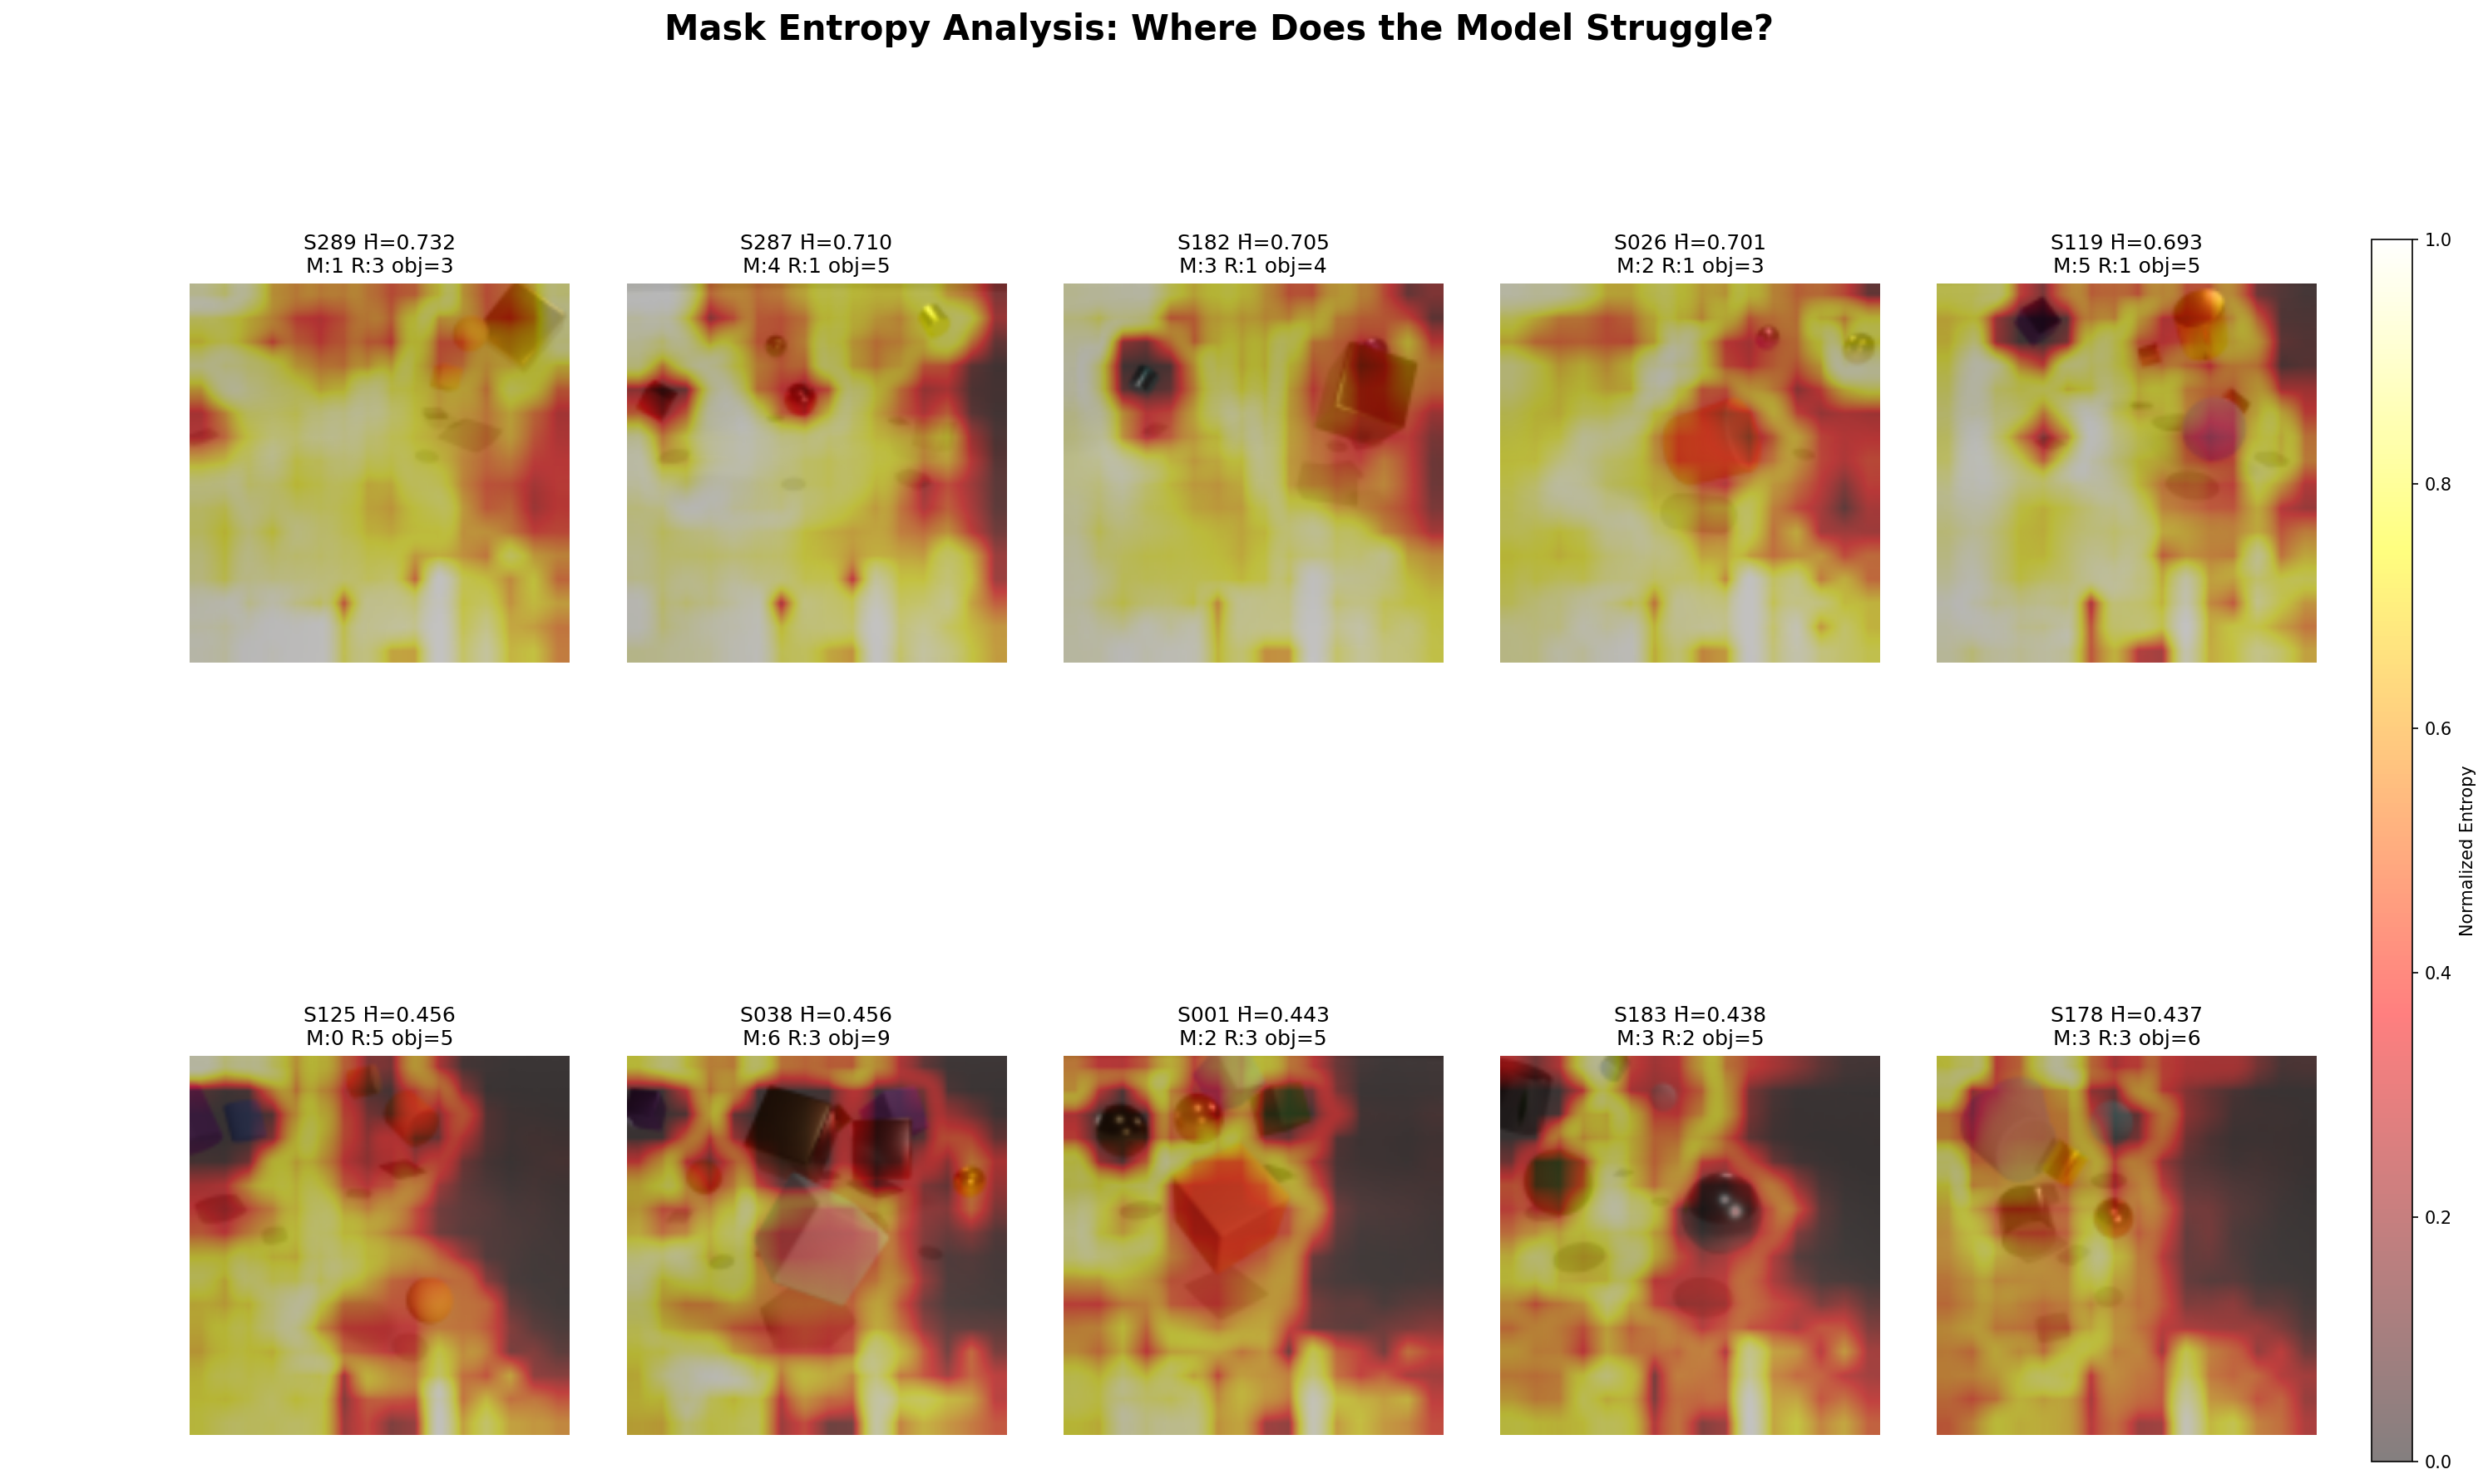
\includegraphics[width=\linewidth,keepaspectratio]{figures/uncertainty_showcase.png}\\[1mm]
\figcap{図7: per-pixelエントロピーマップ（黄=高不確実性）．物体境界で競合が集中 $\Rightarrow$ 物理的境界と一致}
\end{center}

\begin{itemize}[noitemsep,topsep=1mm]
\item 300シーン平均：$\bar{H} = 0.574 \pm 0.056$（範囲 0.44--0.73）
\item 物体数とエントロピーに\textbf{有意な負の相関}：$r{=}{-}0.286$,\;$p{=}4.6{\times}10^{-7}$
\item 余剰スロット（物体数$\ll K$）が\textbf{背景を過分割} $\Rightarrow$ エントロピー上昇
\item \textbf{最適$K$はデータセット固有}のハイパーパラメータ（物体数EDAが先決）
\end{itemize}

\vspace{2mm}

\sechead{8.\ 時系列追跡の予備実験（今後への橋渡し）}

\begin{center}
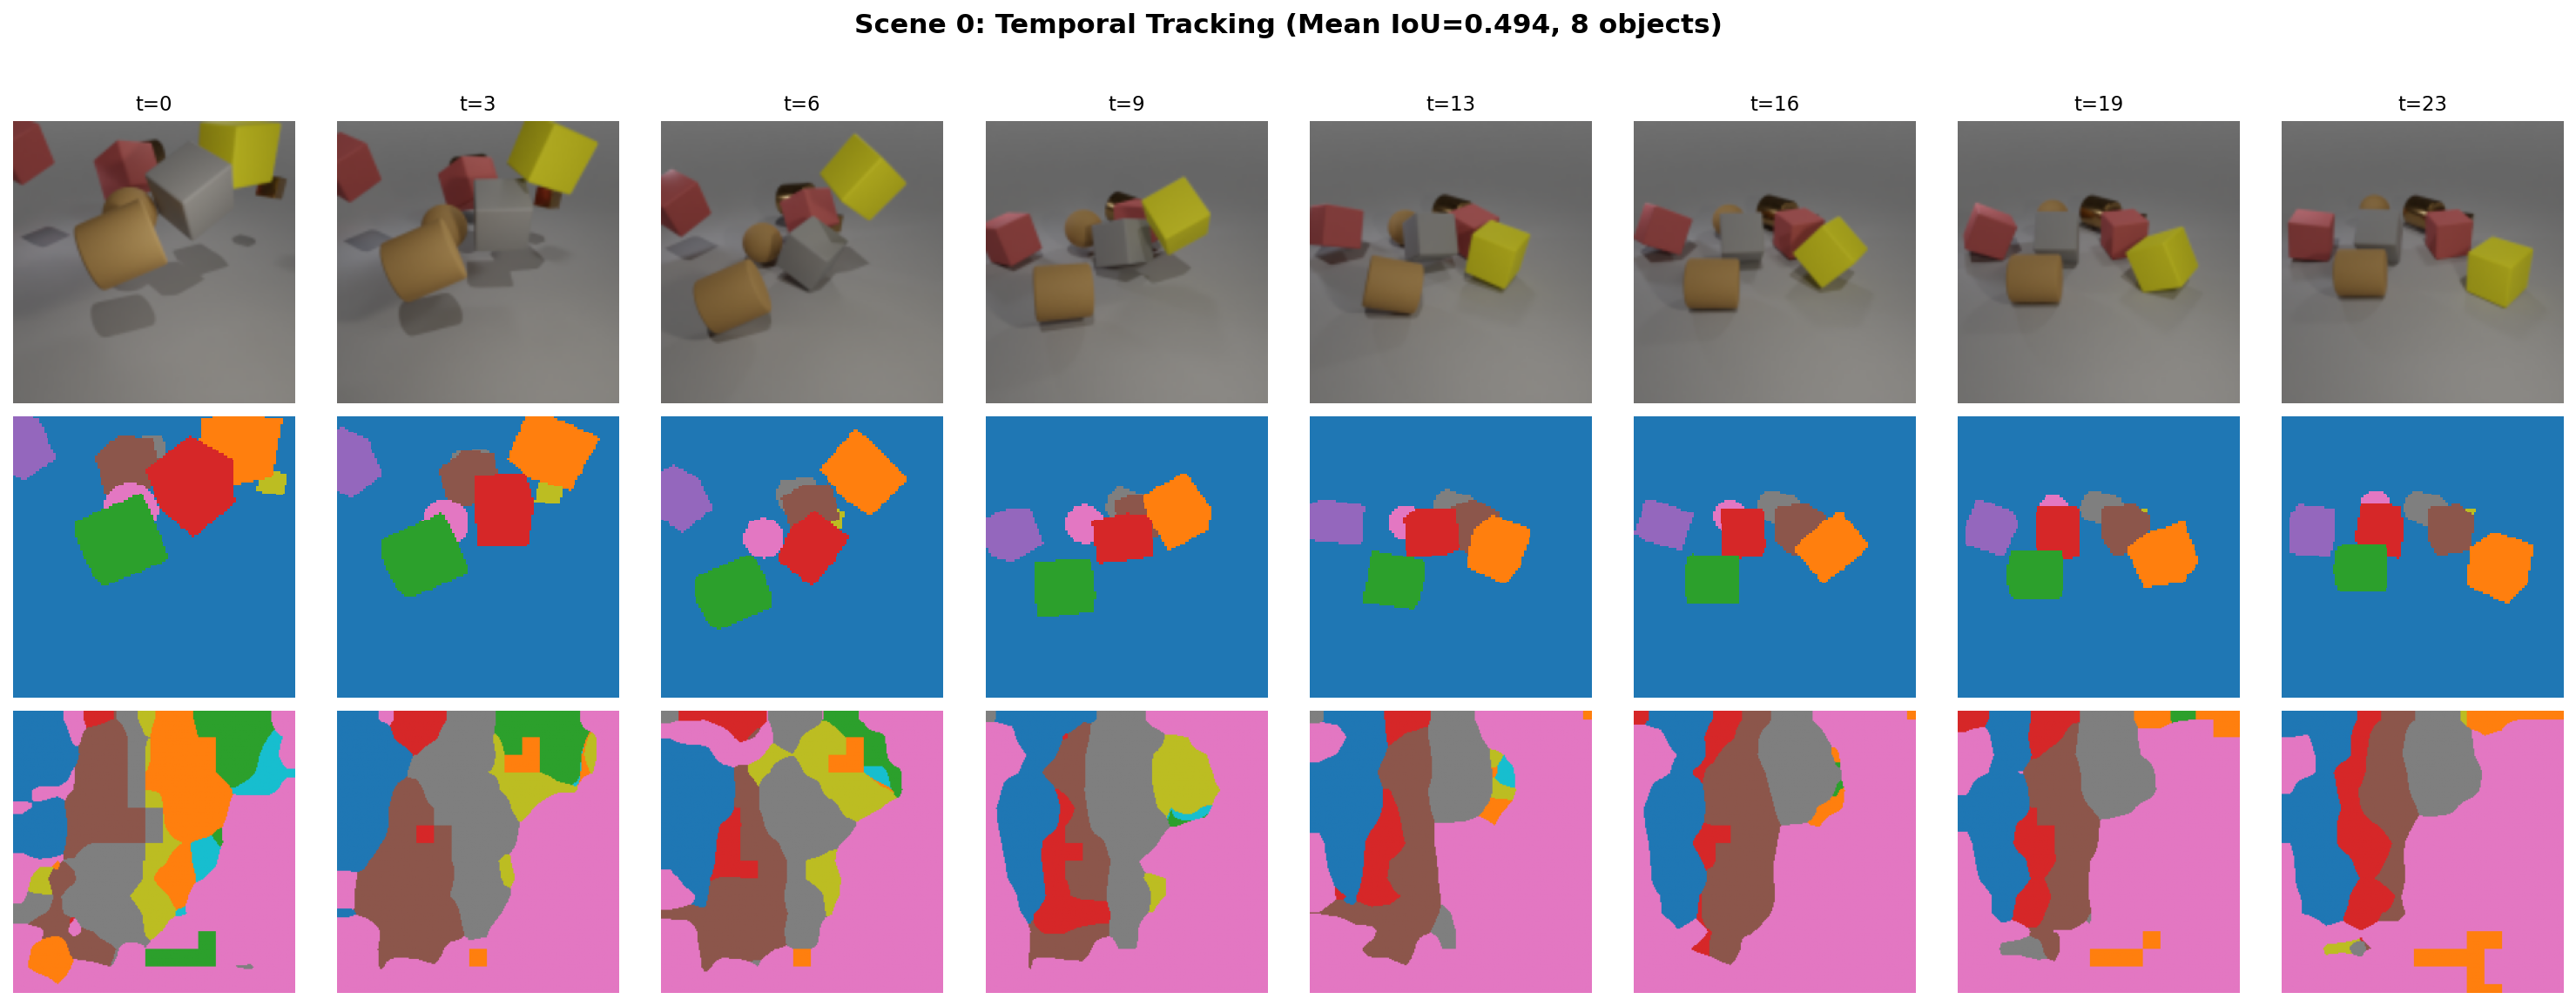
\includegraphics[width=\linewidth,keepaspectratio]{figures/temporal_scene000.png}\\[1mm]
\figcap{図8: Scene 000（IoU=0.494，最良シーン）の時系列セグメンテーション推移．前半で追跡維持，後半でスロット入替り発生}
\end{center}

\begin{itemize}[noitemsep,topsep=1mm]
\item 40シーン$\times$24フレームを\texttt{forward\_video}で処理
\item 平均IoU一貫性：\textbf{0.413 $\pm$ 0.035}（ランダム基準${\approx}0.09$を大幅超）
\item 静止画訓練のみでは\textbf{追跡に限界} $\Rightarrow$ 動画ベース学習が根本解決策
\end{itemize}

\vspace{2mm}

\sechead{9.\ まとめと今後の課題}

\textbf{主要な知見}
\begin{itemize}[noitemsep,topsep=1mm]
\item \textbf{DINOv2 + K=9}でFG-ARI 0.651，448px $\tau$=0.3で\textcolor{darkgreen}{\textbf{0.696}}（全条件最良）
\item DINOv2の成功は\textbf{Goldilocks特性}（3軸の中間値）に起因
\item 金属光沢面の分離：静止画では有意差なし（p=0.12）$\Rightarrow$ \textbf{動画学習}で改善期待
\item 最適$K$はデータセット固有 $\Rightarrow$ \textbf{スロット数EDAが必須前処理}
\end{itemize}

\vspace{1mm}
\textbf{今後の課題}
\begin{itemize}[noitemsep,topsep=1mm]
\item \textbf{動画ベース学習（VideoSAUR型）}でスロットの時間追跡精度を向上
\item DINOv1の救済：投影次元拡大（$>$64）またはPCA前処理
\item Goldilocks特性の実世界画像での再現実験
\end{itemize}

\vspace{1.5mm}
\colorbox{lightyellow}{\parbox{\dimexpr\linewidth-2\fboxsep\relax}{\small%
\textbf{Limitations（批判的視点）}\\
\textbullet\;300サンプル $=$ 先行研究の1/100規模 $\Rightarrow$ スケーリング知見は慎重に\\
\textbullet\;解像度実験は$\tau$と\textbf{交絡} $\Rightarrow$ 独立した制御実験が必要\\
\textbullet\;Goldilocks特性はPCA（線形）計測 $\Rightarrow$ 非線形構造の可能性を排除せず}}

\end{minipage}

\end{document}
